\documentclass[aspectratio=169, compress]{beamer}
\usetheme{Warsaw}
\setbeamertemplate{headline}{}
\usepackage{tikz}
\usetikzlibrary{backgrounds}
\usepackage{minted}
\usepackage{pdfpages}
\usefonttheme{professionalfonts}
\usecolortheme{sidebartab}
\usepackage{xcolor}
\usepackage{svg}
\usepackage{hyperref}
\usepackage[most]{tcolorbox}
\definecolor{bg}{RGB}{210, 255, 180}
\definecolor{aquamarine}{rgb}{0.5, 1.0, 0.83}
\newcommand{\highlight}[1]{\colorbox{pink}{#1}}
\newcommand{\highlightcode}[1]{\colorbox{bg}{#1}}
\newcommand{\highlightflag}[1]{\colorbox{yellow}{#1}}
\newcommand{\colorprog}[1]{\colorbox{aquamarine}{#1}}
\newcommand{\colorpred}[1]{\colorbox{green}{#1}}
\newcommand{\colorinv}[1]{\colorbox{yellow}{#1}}
\newcommand{\coloralg}[1]{\colorbox{pink}{#1}}
\newcommand{\coloryellow}[1]{\colorbox{yellow}{#1}}
\usetikzlibrary{chains, shadows.blur, trees}
%Information to be included in the title page:
\title[Hot Path SSA in LLVM] %optional
{The Hot Path SSA Form in LLVM}

\subtitle{Algorithms \& Applications}

\author[Muzzammil, Mishra, Lahiri, Pandey, and Roy] % (optional, for multiple authors)
{Mohd. Muzzammil\inst{1}, Abhay Mishra\inst{1}, Sumit Lahiri\inst{1} \\ Awanish Pandey\inst{2}, and Subhajit Roy\inst{1}}

\institute[IDK] % (optional)
{
	\inst{1}%
	Dept. of Computer Science \& Engineering,
	IIT Kanpur \\
	\inst{2}%
	Qualcomm India Pvt. Ltd.
}

\date[01/03/2022] % (optional)

\addtobeamertemplate{navigation symbols}{}{%
	\usebeamerfont{footline}%
	\usebeamercolor[fg]{footline}%
	\hspace{-50em}%
	\raisebox{20pt}[0pt][0pt]{\small{pg.\insertpagenumber}}
}
\setbeamercolor{footline}{fg=red}
\setbeamerfont{footline}{series=\bfseries}

\AtBeginSection[]
{
	\begin{frame}<beamer>
		\frametitle{Presentation Outline}
		\tableofcontents[
			currentsection,
			currentsubsection
		]
	\end{frame}
}

\AtBeginSubsection[]
{
	\begin{frame}<beamer>
		\frametitle{Presentation Outline}
		\tableofcontents[
		currentsection,
		currentsubsection
		]
	\end{frame}
}

\begin{document}
\frame{\titlepage}
\begin{frame}
	\frametitle{References}
	\tcbset
	{
		enhanced,
		left=2mm,
		right=2mm,
		boxrule=0.4pt,
		colback=red!5!white,
		boxrule=1.2pt,
		colframe=red!75!black,fonttitle=\bfseries,
	}
	\begin{tcolorbox}[colback=red!3!white,colframe=red!50!black,lifted shadow={1mm}{-2mm}{3mm}{0.1mm}{black!50!white}]
		This presentation presents the details of building a robust and efficient implementation of the \textbf{Hot Path SSA (HPSSA)} form in the LLVM compiler infrastructure. 
	\end{tcolorbox}
	\pause \vspace{10pt}
	The Hot Path SSA form is based on the following research papers.
	\vspace{15pt}
	\begin{itemize}
		\setlength\itemsep{1em} 
		\item Subhajit Roy and Y.N. Srikant. The Hot Path SSA Form: Extending the Static Single Assignment Form for Speculative Optimizations. In CC '10: International Conference on Compiler Construction. 2010. \href{https://link.springer.com/chapter/10.1007/978-3-642-11970-5_17}{CC 2010:304-323} 
		\item Smriti Jaiswal, Praveen Hegde and Subhajit Roy. Constructing HPSSA over SSA. In Proceedings of the 20th International Workshop on Software and Compilers for Embedded Systems. 2017.
		\href{https://dl.acm.org/doi/10.1145/3078659.3078660}{SCOPES 2017: 31-40}
	\end{itemize}
\end{frame}
\footnotesize
\section{HPSSA : Why another SSA Form?}
\subsection{Introduction to Path Profile Guided Optimizations}
{
	\setbeamercolor{background canvas}{bg=}
	\includepdf[pages={5,6,7,8,9,10,11}]{summary.pdf}
}
\begin{frame}
	\frametitle{Why is path-profile-guided analysis hard?}
	\tcbset
	{
		enhanced,
		left=2mm,
		right=2mm,
		boxrule=0.4pt,
		colback=red!5!white,
		boxrule=1.2pt,
		colframe=red!75!black,fonttitle=\bfseries,
	}
	\begin{tcolorbox}[colback=red!3!white,colframe=red!50!black,lifted shadow={1mm}{-2mm}{3mm}{0.1mm}{black!50!white}]
	disparate data-structures, one for \textbf{program representation} and other for \textbf{profile information}.
	\end{tcolorbox}
	\centering
	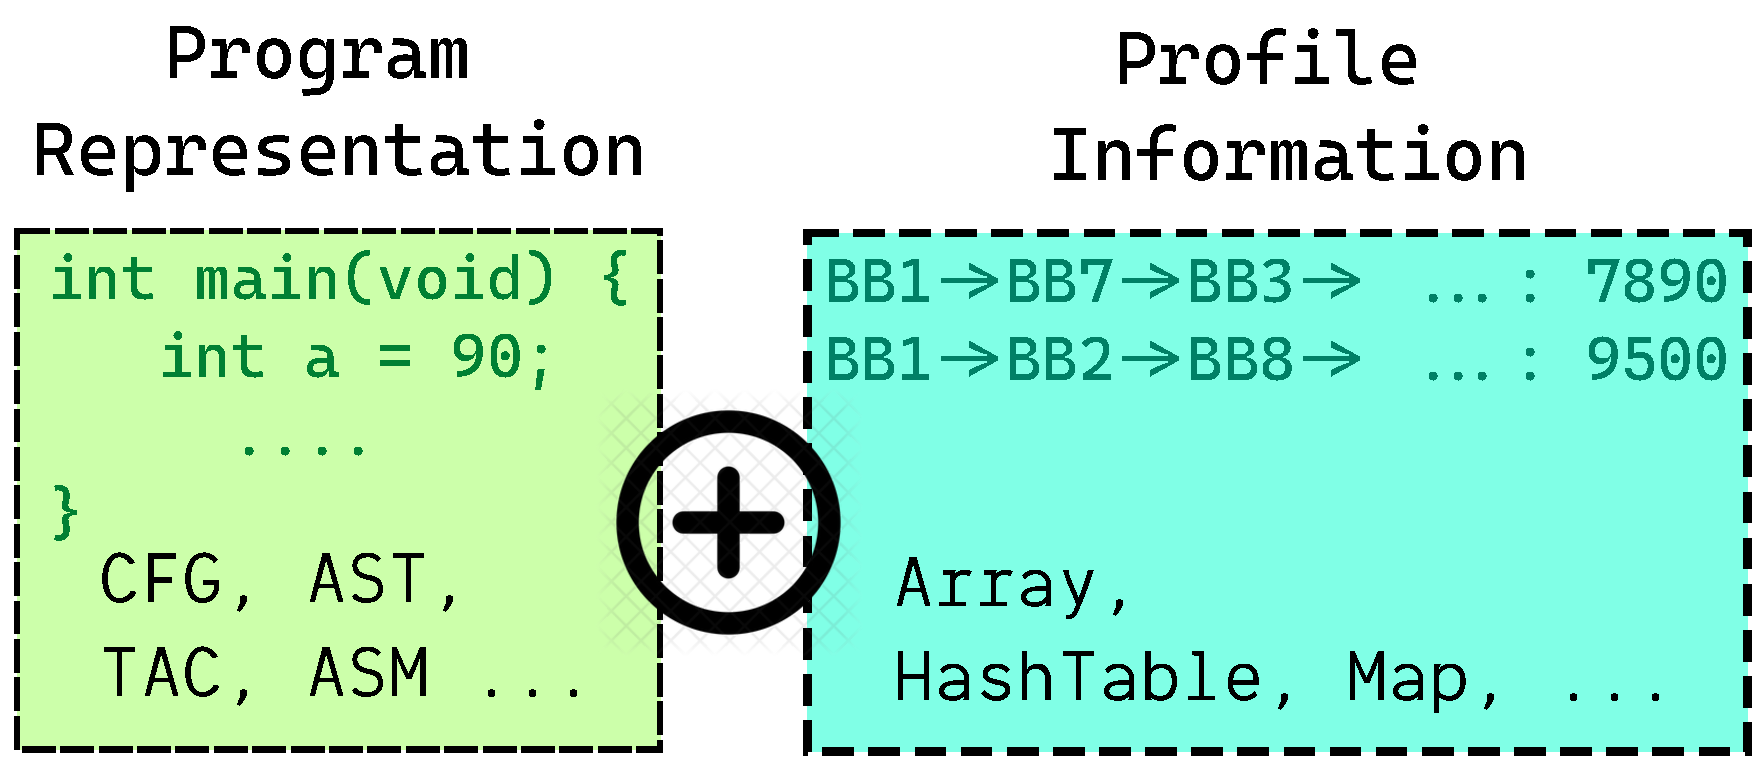
\includegraphics[width=11.5cm, height=5cm]{dotfiles/docs.pdf}
\end{frame}
{
	\setbeamercolor{background canvas}{bg=}
	\includepdf[pages={18}]{summary.pdf}
}
{
	\setbeamercolor{background canvas}{bg=}
	\includepdf[pages={19,20,21,22}]{summary.pdf}
}
\begin{frame}[fragile]
	\frametitle{... and PGO is easy with the Hot Path SSA (HPSSA) Form!}
	\begin{columns}
		\begin{column}{0.5\textwidth}
	\begin{minted}[xleftmargin=1.2em, tabsize=2, numbersep=0.4em, fontsize=\tiny, linenos, highlightcolor=yellow, highlightlines={1},escapeinside=||]{cpp}
// Function to process "llvm.tau" function intrinsic.
void SpecSCCPInstVisitor::visitTauNode(Instruction &Tau) {
	// Code similar to that in visitPHINode(...).
	if (Tau.getType()->isStructTy())
    	return (void)markOverdefined(&Tau);
	if (TauState.isOverdefined())
		return (void)markOverdefined(&Tau);
	// additional code.
	unsigned NumActiveIncoming = 0;
	SpecValueLatticeElement &TauState = getValueState(&Tau), 
		beta = getValueState(Tau.getOperand(1)), 
		x0 = getValueState(Tau.getOperand(0));
	
	for (unsigned i = 1, e = (Tau.getNumOperands() - 1); i != e; ++i){
		SpecValueLatticeElement IV = getValueState(Tau.getOperand(i));
		beta.mergeIn(IV);
		NumActiveIncoming++;
		if (beta.isOverdefined())
			break;
	}
	 
	if (beta.isConstantRange() 
			&& beta.getConstantRange().isSingleElement())
		beta.markSpeculativeConstantRange(beta.getConstantRange());
	if (beta.isConstant())
		beta.markSpeculativeConstant(beta.getConstant());
		
	|\colorprog{x0.mergeInSpec(beta, TauState)};|
	... // futher processing similar to visitPHINode();
}
\end{minted}
		\end{column}
	\begin{column}{0.01\textwidth} \end{column}
		\begin{column}{0.4\textwidth}  
			\begin{minted}[fontsize=\tiny, xleftmargin=1em, tabsize=2, numbersep=0.5em, linenos, highlightcolor=yellow, highlightlines={1,2,13}, escapeinside=||]{cpp}
// Omit handling of "llvm.tau" intrinsic 
// as a regular Instruction.
void SpecSCCPInstVisitor::solve() {
	...
	...
	for (auto& I : *&(*(BB))) {
		CallInst* CI = dyn_cast<CallInst>(&I);
		if (CI != NULL) {
			Function* CF = CI->getCalledFunction();
			if (CF != NULL &&
				CF->getIntrinsicID() == 
			  Function::lookupIntrinsicID("llvm.tau")){
				visitTauNode(I);
			} else {
				visit(I);
			} 
		} else {
			visit(I);
		}
	}
	... // rest of the code.
}

			\end{minted}
		\end{column}
	\end{columns}
\begin{tikzpicture}[remember picture, overlay]
	% we don't want to affect the bounding box if the rectangle is too large
	\begin{pgfinterruptboundingbox}
		% the following coords. may need to be changed to suit your slides
		\fill <2> [fill=white, opacity=0.8] (-2,0) rectangle (16,7.5);
		\fill <3> [fill=white, opacity=0.8] (-2,0) rectangle (16,7.5);
	\end{pgfinterruptboundingbox}
	\node <2> [rectangle,
		rounded corners,
		shade,
		top color=blue!10,
		bottom color=blue!30,
		inner xsep=-35pt,
		inner ysep=3pt,
		text width=\columnwidth,
		text centered,
		anchor=center
		] at (7, 4) {%
		Only these \textbf{few lines} were enough to create a \textbf{new path profile guided analysis}, \\ \textit{Speculative Sparse Conditional Constant Propagation (SpecSCCP)} \\ from the currently existing SCCP pass in LLVM !
	};
	\node <3> [rectangle,
		rounded corners,
		shade,
		top color=red!5,
		bottom color=red!20,
		inner xsep=-8pt,
		inner ysep=5pt,
		text width=30em,
		text centered,
		anchor=center
		] at (7,4) {%
			\textbf{It took us only an afternoon to transform SCCP to SpecSCCP} 
		};
\end{tikzpicture}
\end{frame}
%Slide-1
%Only these few lines were enough to create a new path profile guided analysis, \textit{speculative sparse conditional constant propagation (SpecSCCP)} from the currently existing SCCP pass in LLVM!
%Slide-2
%It took us only an afternoon to transform SCCP to SpecSCCP!.  
\subsection{Profile Guided SpecSCCP Analysis using HPSSA Form}
\begin{frame}[fragile]
	\frametitle{SCCP vs SpecSCCP}
	\begin{columns}
		\begin{column}{0.4\textwidth}
			\fbox{SCCP}
			\begin{minted}[fontsize=\tiny, xleftmargin=1em, tabsize=2, numbersep=0.5em, linenos, highlightcolor=yellow, highlightlines={}, escapeinside=||]{cpp}
int main() {
	int x = 2, m, n, y, z = 9, c = 1;
	std::cin >> |\coloralg{m}|;
	switch(|\coloralg{m}|) {   
		case 2 : |\coloryellow{x}| = 2 * |\coloryellow{c}| + 5; |\coloryellow{n}| = 10; break;
		case 4 : |\coloryellow{x}| = 2 * |\coloryellow{c}| + 5; |\coloryellow{n}| = |\coloralg{x}| - 2; break;
		case 6 : |\coloryellow{x}| = 2 * |\coloryellow{c}| + 1; |\coloryellow{n}| = |\coloralg{x}| + 2; break;
		default : break;
	}
	|\coloralg{y}| = 2 * |\coloralg{x}| + 10;
	if (|\coloralg{y}| <= |\coloralg{z}| + |\coloralg{x}|) {
		// ..
	} else {
		|\coloralg{z}| = |\coloralg{n}| + 3 * |\coloralg{x}|;
		switch (|\coloralg{z}|) {
			default : break;
			case 200 : goto end;
			case 300 : exit(0); }
	}
	|\coloralg{m}| = |\coloralg{n}| + |\coloralg{x}|;  
	end:
		|\coloralg{z}| = |\coloralg{x}|;
	return 0;
}
			\end{minted}
		\end{column}
		\begin{column}{0.4\textwidth}
			\fbox{SpecSCCP}  
			\begin{minted}[fontsize=\tiny, xleftmargin=1em, tabsize=2, numbersep=0.5em, linenos, highlightcolor=yellow, highlightlines={}, escapeinside=||]{cpp}
int main() {
	int x = 2, m, n, y, z = 9, c = 1;
	std::cin >> |\coloralg{m}|;
	switch(|\coloralg{m}|) {   
		case 2 : |\coloryellow{x}| = 2 * |\coloryellow{c}| + 5; |\coloryellow{n}| = 10; break;
		case 4 : |\coloryellow{x}| = 2 * |\coloryellow{c}| + 5; |\coloryellow{n}| = |\coloralg{x}| - 2; break;
		case 6 : |\coloryellow{x}| = 2 * |\coloryellow{c}| + 1; |\coloryellow{n}| = |\coloralg{x}| + 2; break;
		default : break;
	}
	|\coloralg{y}| = 2 * |\coloralg{x}| + 10;
	if (|\coloralg{y}| <= |\coloralg{z}| + |\coloralg{x}|) {
		// ..
	} else {
		|\coloralg{z}| = |\colorpred{n}| + 3 * |\coloralg{x}|; // n : Speculative Constant 5
		switch (|\coloralg{z}|) {
			default : break;
			case 200 : goto end;
			case 300 : exit(0); }
	}
	|\coloralg{m}| = |\coloralg{n}| + |\colorpred{x}|;  // x : Speculative Constant 7
	end:
		|\coloralg{z}| = |\coloralg{x}|;
	return 0;
}
		\end{minted}
		\end{column}
	\end{columns}
	\vspace{1pt}
	\fbox{\textbf{Legend:} \textcolor{pink}{$\blacksquare$} Overdefined \textcolor{yellow}{$\blacksquare$} Real Constants
	\textcolor{green}{$\blacksquare$} Speculative Constants}
\begin{tikzpicture}[remember picture, overlay]
	% we don't want to affect the bounding box if the rectangle is too large
	\begin{pgfinterruptboundingbox}
		% the following coords. may need to be changed to suit your slides
		\fill <2> [fill=white, opacity=0.8] (-100,-1) rectangle (16, 7.8);
	\end{pgfinterruptboundingbox}
	\node <2> [rectangle,
	rounded corners,
	shade,
	top color=blue!5,
	bottom color=blue!20,
	inner xsep=-15pt,
	inner ysep=5pt,
	text width=30em,
	text centered,
	anchor=center
	] at (-3, 4) {%
		\textbf{SpecSCCP discovers $n$ \& $x$ as speculative constants.}
	};
\end{tikzpicture}
\end{frame}
%Slide-3
%(SpecSCCP discovers n & x as speculative constants.)
\begin{frame}
	\centering
	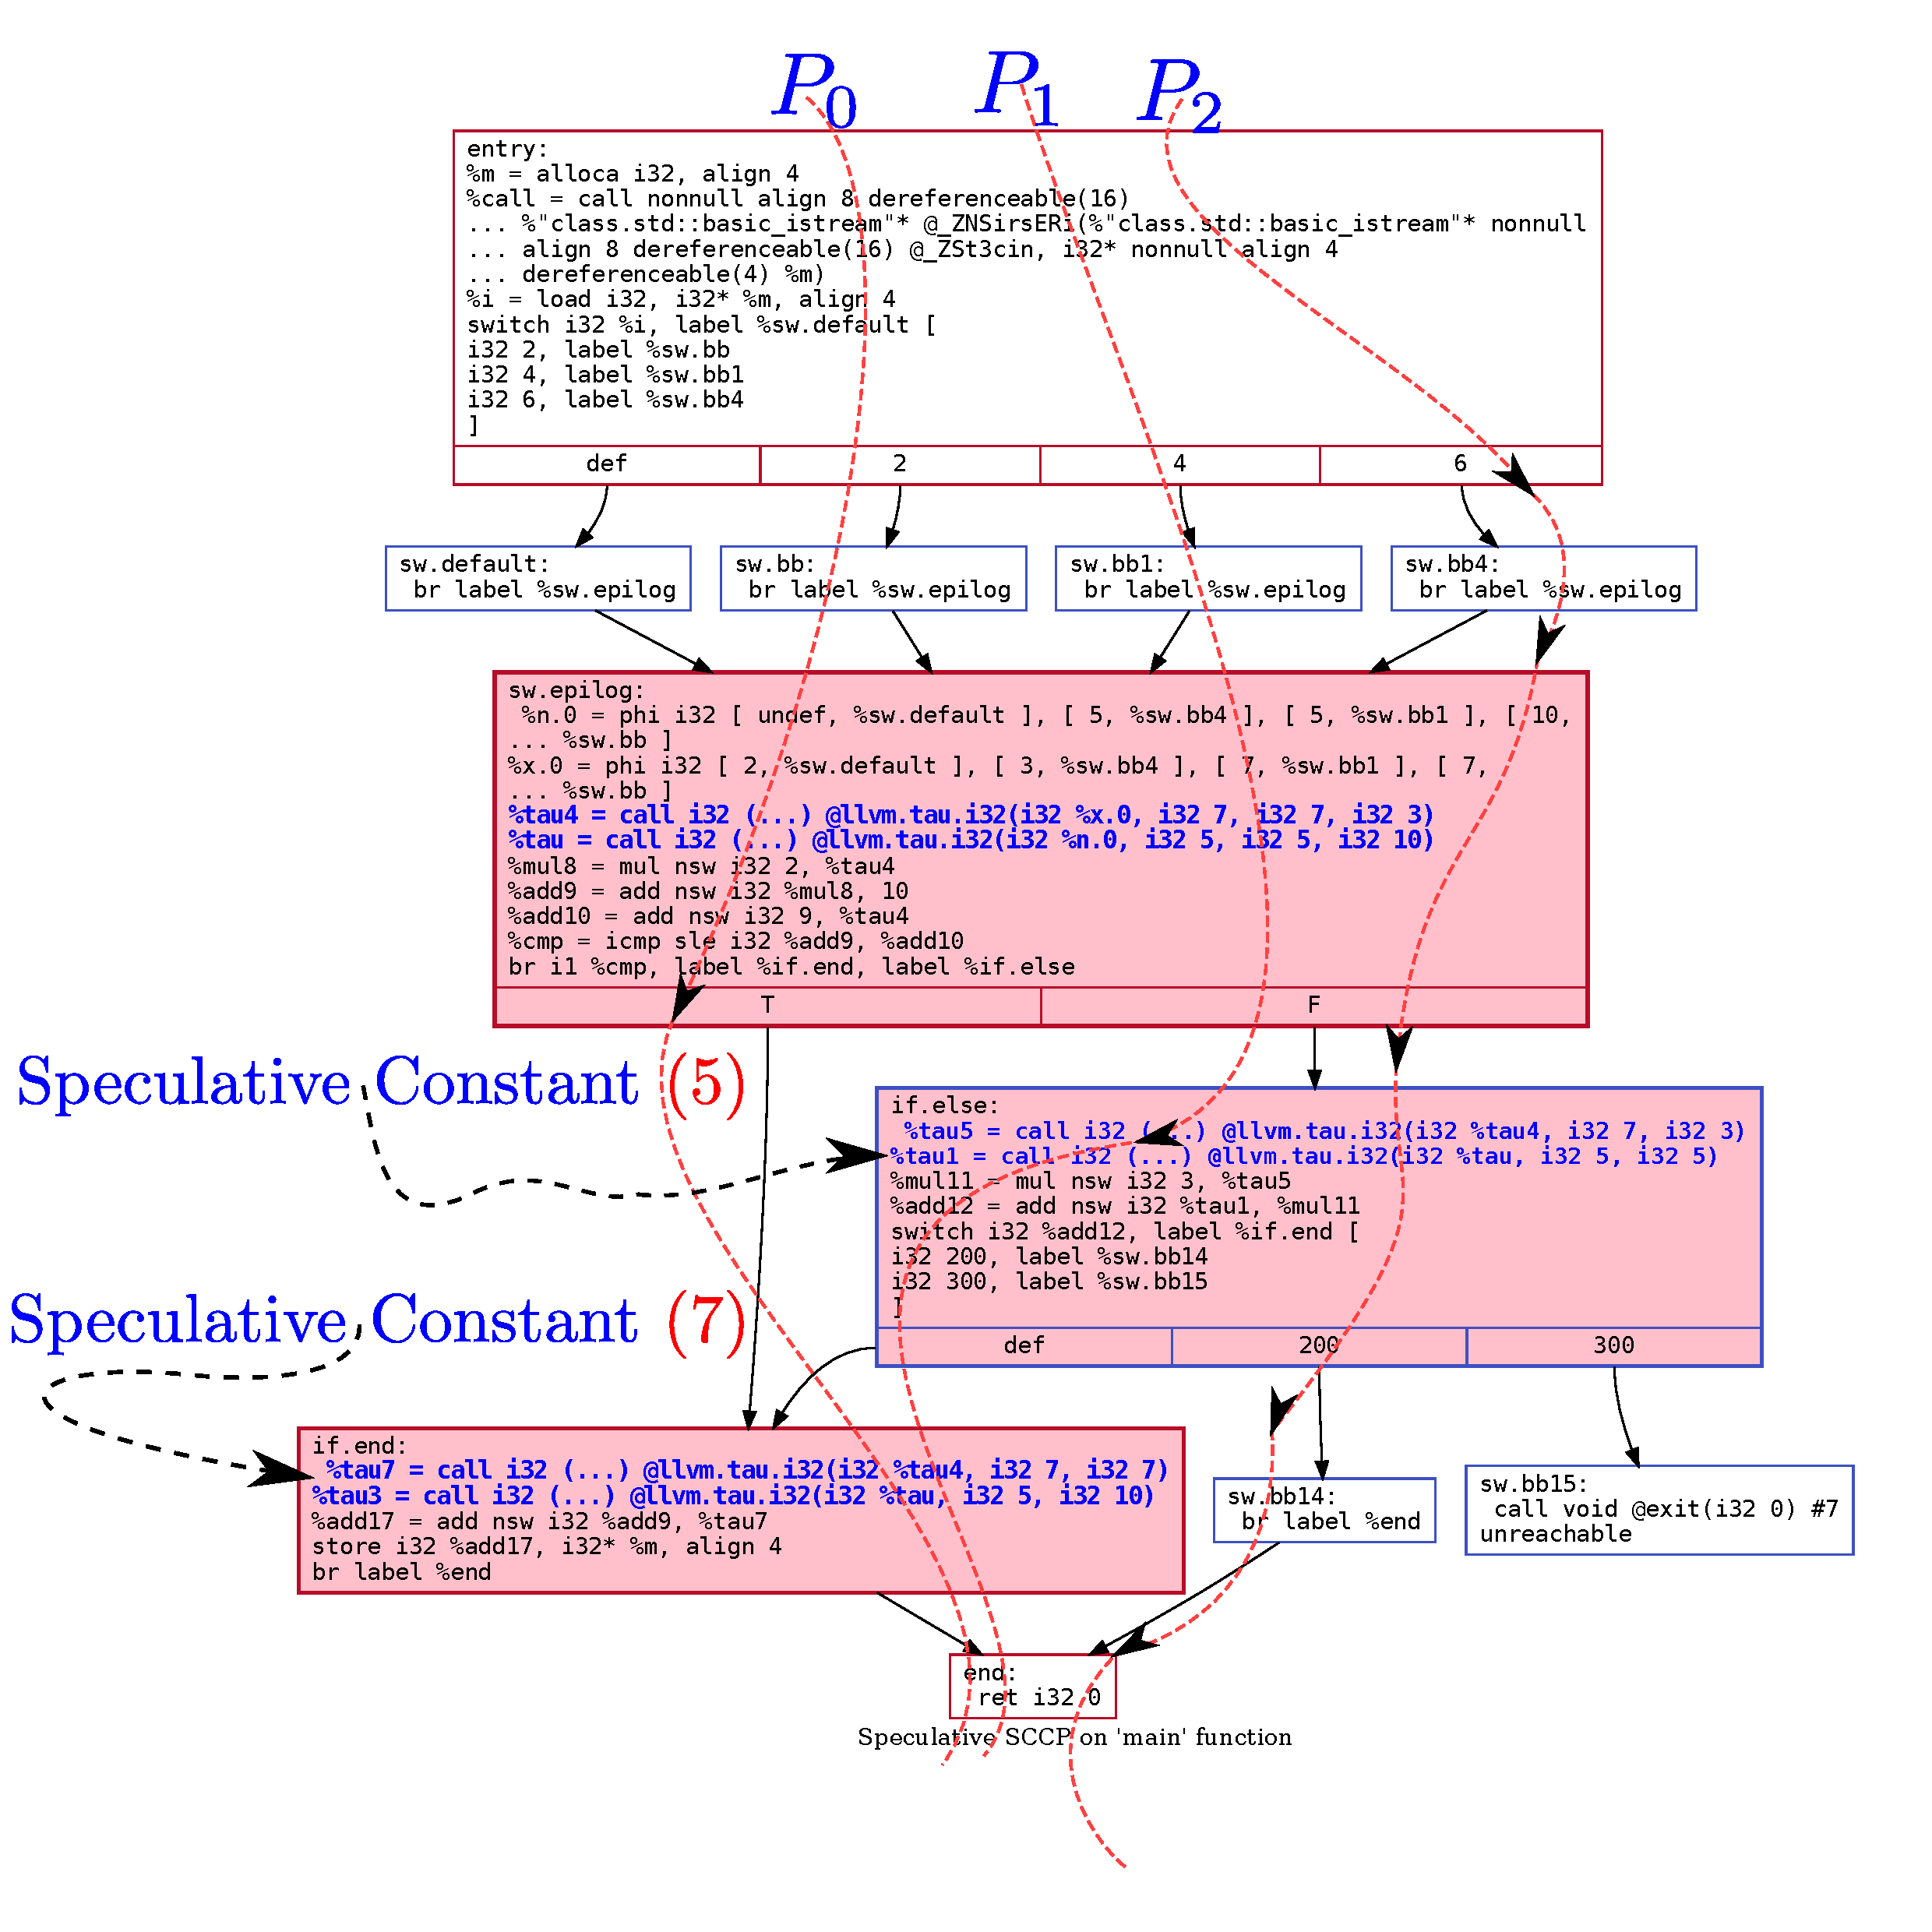
\includegraphics[width=10cm, height=9.5cm]{dotfiles/specSCCP_HPSSA_prev.dot.pdf}
\end{frame}
\begin{frame}
	\centering
	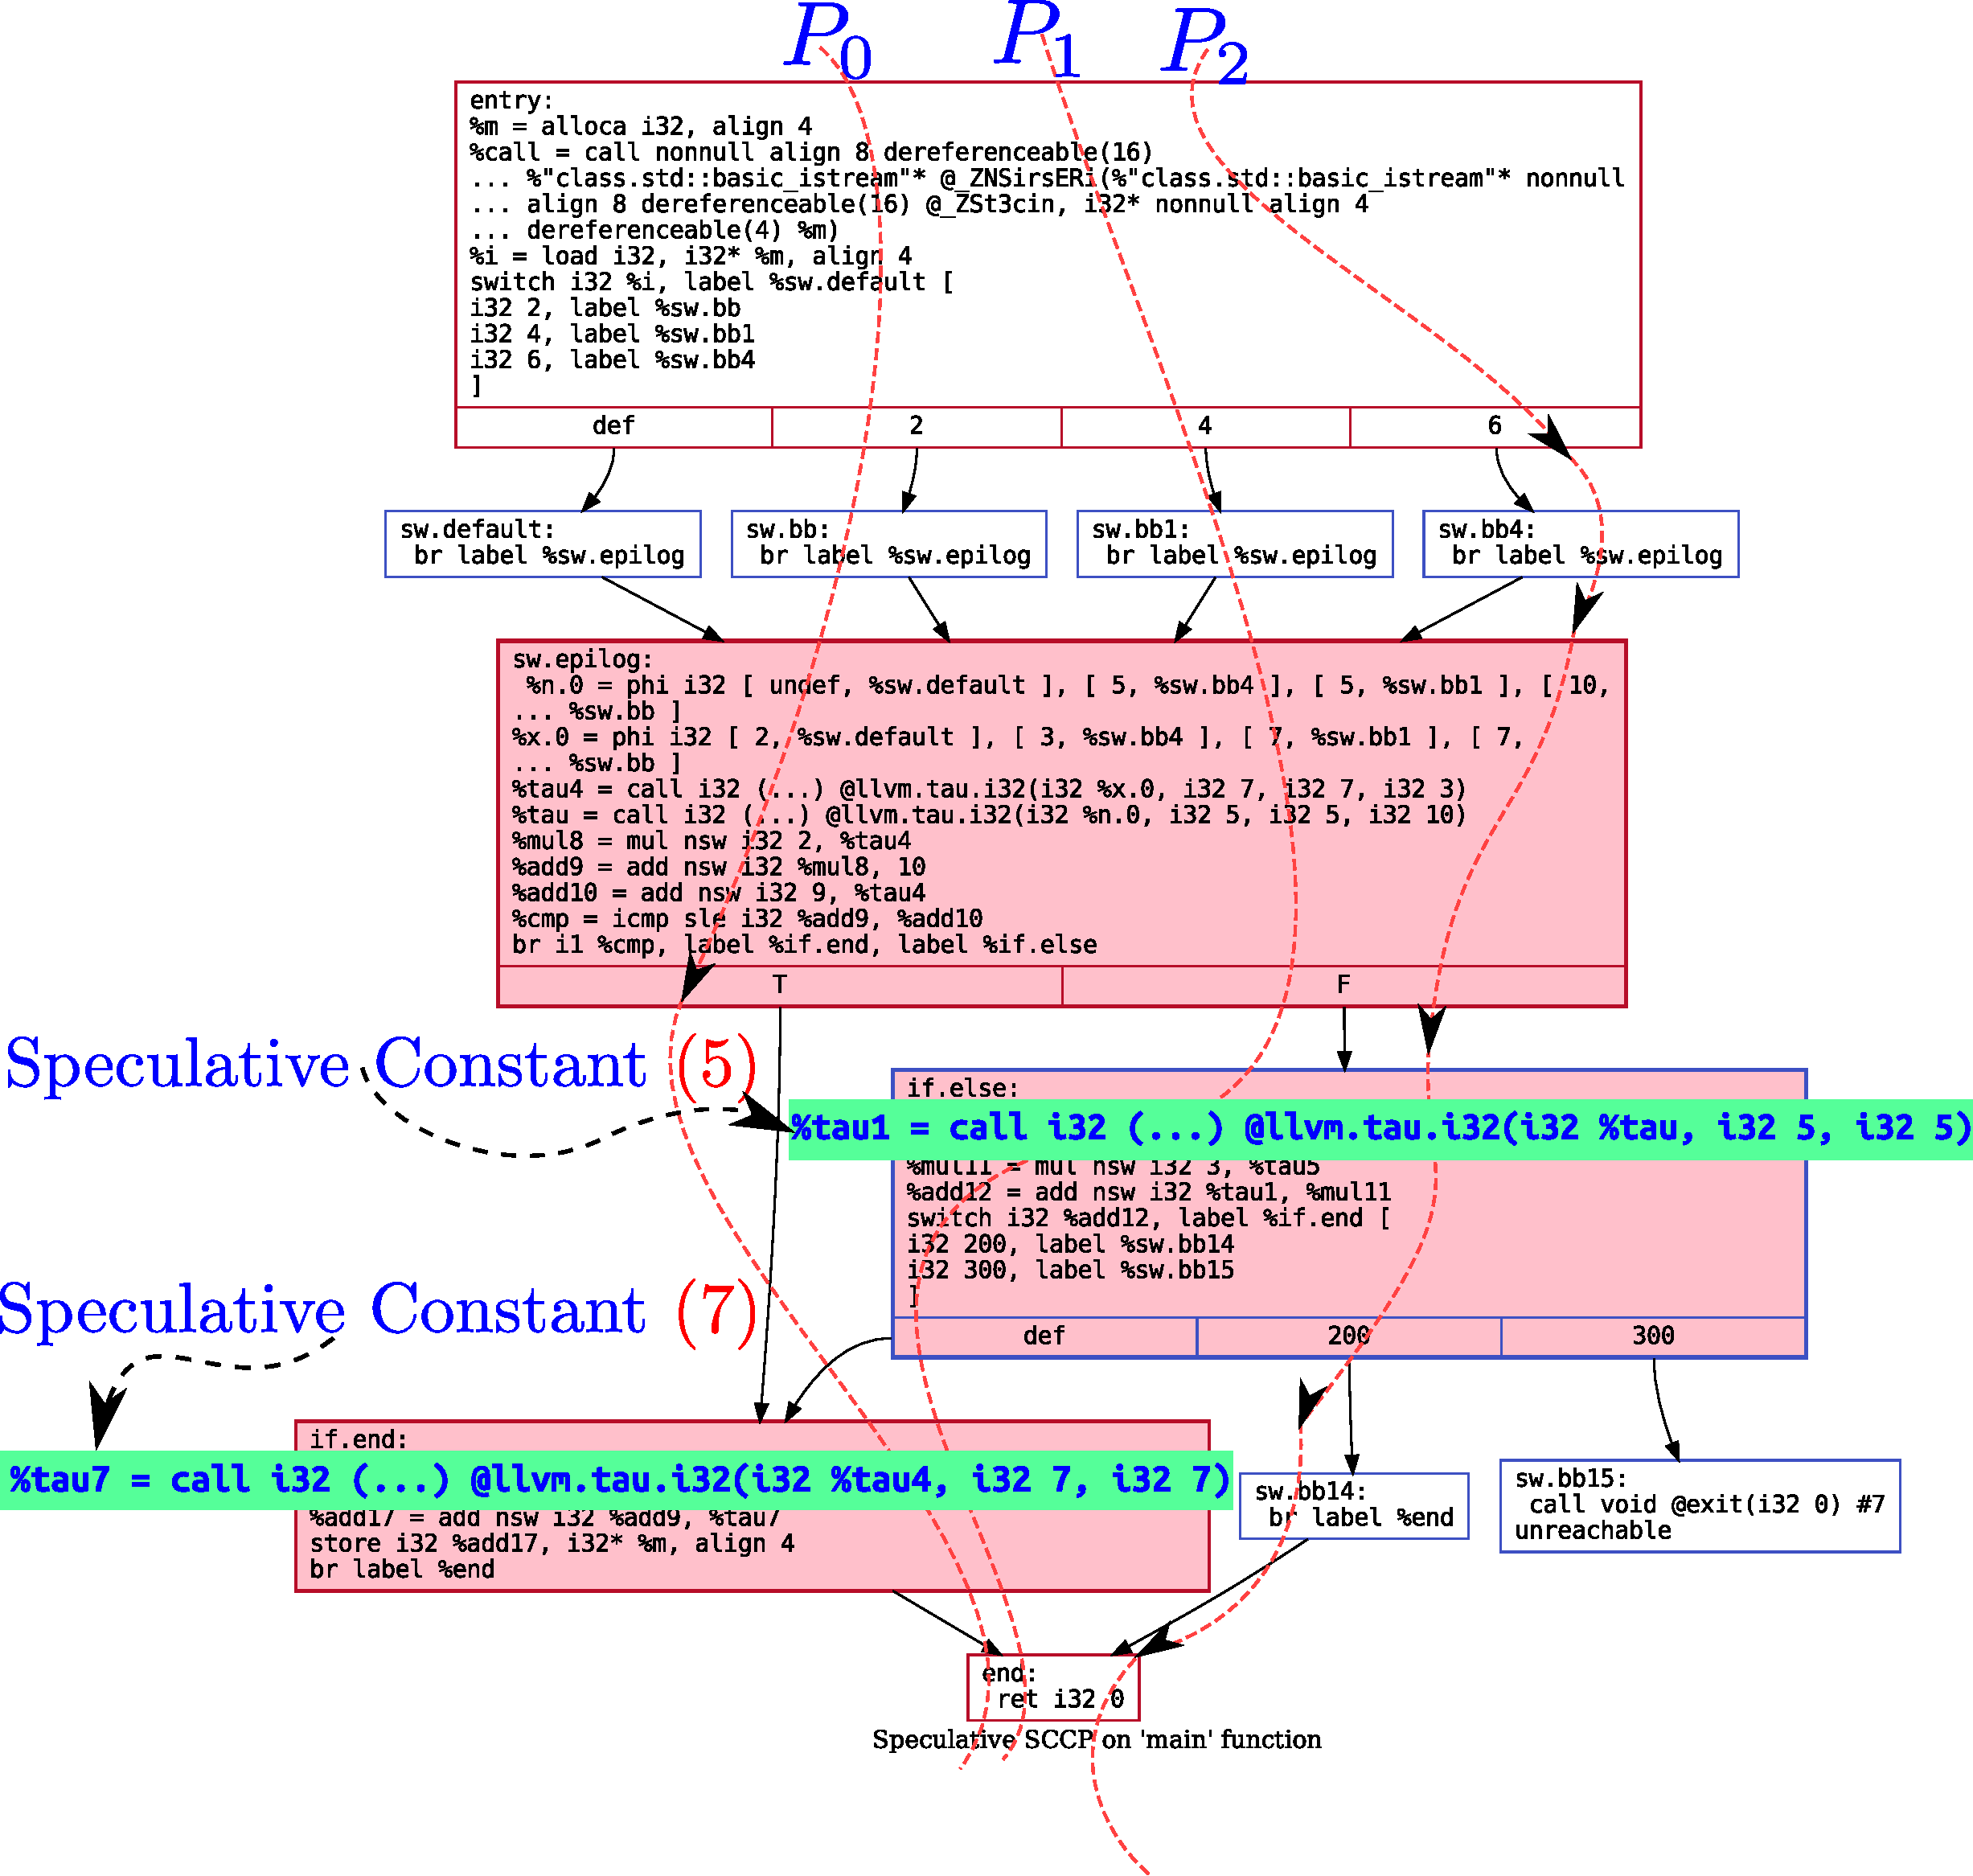
\includegraphics[width=10.2cm, height=9.5cm]{dotfiles/specSCCP_HPSSA_next.dot.pdf}
\end{frame}
\begin{frame}[fragile]
	\frametitle{SCCP vs SpecSCCP}
	Standard SCCP VS. Speculative SCCP Pass.
\begin{columns}
	\begin{column}{0.4\textwidth}
		\begin{minted}[fontsize=\tiny, tabsize=2, linenos, highlightcolor=yellow, highlightlines={}]{c}
# Running Regular SCCP Pass on Program.
$ opt -sccp -time-passes -debug-only=sccp \
	IR/LL/test.ll -S -o \
	IR/LL/test_sccp_onbaseline.ll \
	-f 2> output/custom_sccp_onbaseline.log

...
Output:
	...
	Constant: i32 2 =   %mul = mul nsw i32 2, 1
	Constant: i32 7 =   %add = add nsw i32 2, 5
	Constant: i32 2 =   %mul2 = mul nsw i32 2, 1
	Constant: i32 7 =   %add3 = add nsw i32 2, 5
	Constant: i32 5 =   %sub = sub nsw i32 7, 2
	Constant: i32 2 =   %mul5 = mul nsw i32 2, 1
	Constant: i32 3 =   %add6 = add nsw i32 2, 1
	Constant: i32 5 =   %add7 = add nsw i32 3, 2
	
	
	
	
		\end{minted}
	\end{column}
	\begin{column}{0.5\textwidth}  
		\begin{minted}[fontsize=\tiny, tabsize=2, linenos, highlightlines={3,20,21,22,23}]{c}
# Running HPSSA Transformation followed by Speculative SCCP Pass.
$ opt -load build/SCCPSolverTau.cpp.so 
	-load build/HPSSA.cpp.so \
	-load-pass-plugin=build/SpecSCCP.cpp.so \
	-passes="specsccp" \
	-time-passes -debug-only=specsccp \
	IR/LL/test.ll -S -o IR/LL/test_spec_sccp.ll \
	-f 2> output/custom_speculative_sccp.log
	
...
Output :
	Constant: i32 2 =   %mul = mul nsw i32 2, 1
	Constant: i32 7 =   %add = add nsw i32 2, 5
	Constant: i32 2 =   %mul2 = mul nsw i32 2, 1
	Constant: i32 7 =   %add3 = add nsw i32 2, 5
	Constant: i32 5 =   %sub = sub nsw i32 7, 2
	Constant: i32 2 =   %mul5 = mul nsw i32 2, 1
	Constant: i32 3 =   %add6 = add nsw i32 2, 1
	Constant: i32 5 =   %add7 = add nsw i32 3, 2
Speculative Constant: i32 5 = %tau1 = call i32 (...) 
		@llvm.tau.i32(i32 %tau, i32 5, i32 5)
Speculative Constant: i32 7 = %tau7 = call i32 (...) 
		@llvm.tau.i32(i32 %tau4, i32 7, i32 7)
		\end{minted}
	\end{column}
\end{columns}
\end{frame}
\begin{frame}[fragile]
	\frametitle{Using the HPSSA Form for writing new analyses}
	\begin{itemize}
		\item Include the header file \mintinline[]{python}{HPSSA.h} to use  \mintinline[]{css}{llvm::HPSSAPass} class.
		\item Load shared object using opt tool. \mintinline[]{css}{opt -load HPSSA.cpp.so ...} 
	\end{itemize}
	\begin{minted}[fontsize=\footnotesize, xleftmargin=1em, tabsize=2, numbersep=0.5em, highlightlines={1,12,13}, linenos]{cpp}
#include <HPSSA.h> // import the header.
#include <SCCP.h>

class YourPGOPass : public PassInfoMixin<YourPGOPass> {
	public: PreservedAnalyses run(Function &F, 
	FunctionAnalysisManager &AM);
};

PreservedAnalyses YourPGOPass::run(Function &F, 
	FunctionAnalysisManager &AM) {
		...
		HPSSAPass hpssaUtil; // Make a HPSSAPass Object.
		hpssaUtil.run(F, AM);  // Call the HPSSAPass::run() function.
		...
		// Rest of the code ..
	}
	\end{minted}
%\fbox{
%	Output : \mintinline[]{css}{
%		Total Tau Instructions : 7,
%	...rest of the logs}
%}
\end{frame}
\section{What is HPSSA form?}
\subsection{Hot Path SSA Form}
{
	\setbeamercolor{background canvas}{bg=}
	\includepdf[pages={25,27,28,29,30}]{summary.pdf}
}
\subsection{Profile Guided SpecSCCP Pass}
{
	\setbeamercolor{background canvas}{bg=}
	\includepdf[pages={31,32}]{summary.pdf}
}
\begin{frame}[fragile]
	\frametitle{From \texttt{SpecSCCP} Pass}
	Basic blocks from the transformed IR after the \texttt{SpecSCCP} pass with \texttt{assignSpecValue()} calls added.
	\begin{minted}[frame=single,framesep=0.1pt,fontsize=\footnotesize, tabsize=2, linenos, highlightlines={3,4}, escapeinside=||]{css}
	if.else:                                          ; preds = %sw.epilog
		%tau = call i32 (...) @llvm.tau.i32(i32 %tau8, i32 7, i32 3)
		|\colorpred{%tau10}| = call i32 (...) @llvm.tau.i32(i32 %tau9, i32 5, i32 5)	
		|\colorpred{%tau10\_spec}| = call i32 @assignSpecValue(i32 5)
		%mul11 = mul nsw i32 3, undef
		%add12 = add nsw i32 |\colorpred{%tau10\_spec}|, %mul11
		switch i32 %add12, label %sw.default13 [
			i32 200, label %sw.bb14
			i32 300, label %sw.bb15
		]
	\end{minted}
	\begin{minted}[frame=single,framesep=0.1pt,fontsize=\footnotesize, tabsize=2, linenos, highlightlines={2,3}, escapeinside=||]{css}
	if.end:                                           ; preds = %sw.epilog, %if.else
		|\colorpred{%tau11}| = call i32 (...) @llvm.tau.i32(i32 %tau8, i32 7, i32 7)
		|\colorpred{%tau11\_spec}| = call i32 @assignSpecValue(i32 7)
		%tau12 = call i32 (...) @llvm.tau.i32(i32 %tau9, i32 5, i32 10)
		%add17 = add nsw i32 undef, |\colorpred{%tau11\_spec}|
		store i32 %add17, i32* %m, align 4
		br label %end
	\end{minted}
\end{frame}
\footnotesize

\section{How is HPSSA Implemented?}
\subsection{Constructing HPSSA Form}
{
	\setbeamercolor{background canvas}{bg=}
	\includepdf[pages={55}]{summary.pdf}
}
{
	\setbeamercolor{background canvas}{bg=}
	\includepdf[pages={52,53,54}]{summary.pdf}
}
\subsection{Implementing HPSSA Form in LLVM}

\begin{frame}[fragile]
	\frametitle{What we modified in LLVM Source?}
	\begin{itemize}
		\item New \mintinline[]{css}{llvm::intrinsic} signature, \mintinline[]{css}{"llvm.tau"} to support addition and removal of $\tau$-functions to the LLVM SSA IR representation. \pause
	\end{itemize}
	\begin{minted}[fontsize=\footnotesize, tabsize=4, linenos]{python}
	+ //===---------- intrinsic for tau ---------------=====//
	+ def int_tau : DefaultAttrsIntrinsic<[llvm_any_ty],
	+                   [llvm_vararg_ty],
	+                   []>;
	\end{minted}
	\pause
	\begin{itemize}
		\item Modified \mintinline[]{css}{Verifier::verifyDominatesUse()} function since we don't want our intrinsic to interfere with \mintinline[]{css}{dominators} computation.  \pause
	\end{itemize}
	\begin{minted}[fontsize=\footnotesize, tabsize=4, highlightlines={4,5,6,7,8,9,10}, linenos]{python}
	+ //===---------- Changes for tau.intrinsic ---------------=====//
	void Verifier::verifyDominatesUse(Instruction &I, unsigned i) {
		Instruction *Op = cast<Instruction>(I.getOperand(i));
		+	if (CallInst *CI = dyn_cast<CallInst>(&I)) {
		+	Function *CallFunction = CI->getCalledFunction();
		+	if (CallFunction != NULL && CallFunction->getIntrinsicID()==
		+		Function::lookupIntrinsicID("llvm.tau")) {
		+			return;
		+		}
		+	}
		...
	\end{minted}
\end{frame}

\begin{frame}
	\frametitle{\texttt{HPSSAPass} : Overview}
	\begin{itemize}
		\item \mintinline[]{css}{class HPSSAPass : public PassInfoMixin<HPSSAPass>}
		\begin{itemize}
			\footnotesize
			\item Implemented \mintinline[]{css}{llvm::HPSSAPass} pass using the new LLVM Pass Manager. 
			\item Function \mintinline[fontsize=\footnotesize]{css}{HPSSAPass::run(Function &F, ...)}  runs over a \mintinline[]{css}{llvm::Function} and inserts \mintinline[]{css}{"llvm.tau"} intrinsic calls with speculative and safe argument at strategic positions in the LLVM IR and handles argument allocation for \mintinline[]{css}{"llvm.tau"} intrinsic calls. \pause
		\end{itemize}
		\item Key HPSSA Data Structures and Functions:  \pause
		\begin{itemize}
			\footnotesize
			\item \fcolorbox{blue}{white}{Hot Path Set using \mintinline[]{css}{llvm::BitVector}} \pause for maintaining \color{red} hot paths \color{black} in the program. \pause
			\item \fcolorbox{blue}{white}{\mintinline[]{css}{std::map<llvm::BasicBlock*, llvm::BitVector> HotPathSet}} \pause used to track \color{red} hot paths \color{black} that pass through a given basic block. \pause
			\item \fcolorbox{blue}{white}{\mintinline[]{css}{std::map<std::pair<llvm::BasicBlock *, Value *>, frame> defAcc}} \pause keeps track of the \color{red} hot \color{black} definitions for a variable that reaches a given basic block. \pause
			\item \fcolorbox{blue}{white}{\mintinline[]{css}{std::map<llvm::Value *, std::vector<llvm::Value *>> renaming_stack}} \pause used to store the most ``recent" tau definition encountered so far corresponding for a tau variable used later in variable renaming phase. \pause
			\item \fcolorbox{blue}{white}{\mintinline[]{css}{HPSSAPass::AllocateArgs(BasicBlock* BB, DomTreeNode& DTN)}} \pause handles argument allocation for $\tau$-functions inserted.
		\end{itemize}
	\end{itemize}
\end{frame}

\begin{frame}
	\frametitle{\texttt{HPSSAPass} : Destruction Pass}
	\begin{itemize}
		\item Out of HPSSA Form. 
		\begin{itemize}
			\item A seperate pass using the new LLVM Pass Manager. \mintinline[]{css}{class TDSTRPass : public PassInfoMixin<TDSTRPass>} \pause
			\item Using \mintinline[fontsize=\footnotesize]{css}{TDSTRPass::run(Function &F, ...)}, we replace all use of existing tau operands with first argument of  \mintinline[]{css}{"llvm.tau"} intrinsic (corresponds to the safe argument) and remove the \mintinline[]{css}{"llvm.tau"} intrinsic calll from the LLVM IR.
			\item The LLVM IR becomes identical to what it was before running the HPSSA Pass. \pause
		\end{itemize}
	\end{itemize}
\begin{figure}[]
	\centering
	\begin{minipage}{0.4\textwidth}
		\centering
	\fbox{$x_3 = \tau(x_0, x_1, x_2)$, $\tau$-function}
	\end{minipage}
	\begin{minipage}{0.4\textwidth}
		\centering
	\fbox{$x_3 = x_0, \quad$ Replace all use of $x_3$ with $x_0$.}
	\end{minipage}
\end{figure}

\end{frame}

\footnotesize

\section{Conclusion}
\begin{frame}
	\frametitle{Conclusion}
	\begin{itemize}
		\item The Hot Path SSA form opens up an exciting opportunity for compiler writers to ``port" exisiting standard analyses to their profile guided variants. \pause
		\item We plan to open source our work soon and push it to the LLVM ``main" branch.
	\end{itemize}
\end{frame}

\begin{frame}
	\frametitle{LLVM Implementation : Profile Guided SpecSCCP Pass}
	\begin{itemize}
		\item Modified the existing SCCP Pass to add \mintinline[fontsize=\footnotesize]{css}{visitTauNode()} function which handles the special \mintinline[fontsize=\footnotesize]{css}{"llvm.tau"} intrinsic instructions used for $\tau$-functions.\footnotemark \pause
		\item Added a new lattice element type \mintinline[fontsize=\footnotesize]{css}{"spec_constant"} and \mintinline[fontsize=\footnotesize]{css}{mergeInSpec()} function in \mintinline[fontsize=\footnotesize]{css}{ValueLattice} class supporting operations on speculative constants. Modified the existing \mintinline[fontsize=\footnotesize]{css}{mergeIn()} function to handle lattice ``meet" operation for the new speculative constants introduced.  \pause
		\item Added new functions in the \mintinline[fontsize=\footnotesize]{css}{SCCPInstVisitor} and \mintinline[fontsize=\footnotesize]{css}{SCCPSolver} class to handle operations on speculative constants. Eg. Operands can be marked speculative using as function \mintinline[fontsize=\footnotesize]{css}{markSpeculativeConstant()}. \pause
		\item Modified the \mintinline[fontsize=\footnotesize]{css}{SCCPInstVisitor::solve()} function to process \mintinline[fontsize=\footnotesize]{css}{"llvm.tau"} intrinsic instructions using \mintinline[fontsize=\footnotesize]{css}{visitTauNode()} instead of the standard \mintinline[fontsize=\footnotesize]{css}{visit()} function.
	\end{itemize}
	\tiny 
	\footnotetext[1]{Since we added the $\tau$-functions as an \mintinline[fontsize=\footnotesize]{css}{"llvm.tau"} intrinsic, we blocked processing it as a regular LLVM Instruction.}
\end{frame}

\begin{frame}
	\frametitle{\texttt{HPSSAPass} : Details of \texttt{run(...)}}
	\begin{itemize}
		\item \mintinline[fontsize=\footnotesize]{cpp}{HPSSAPass::run(Function &F, FunctionAnalysisManager &AM)} 
		\begin{itemize}
			\footnotesize
			\item Invokes \mintinline[fontsize=\footnotesize]{css}{HPSSAPass::getProfileInfo()} function to get a compact representation of all the profiled \color{red} hot paths \color{black} in the program and then calls \mintinline[fontsize=\footnotesize]{css}{HPSSAPass::getCaloricConnector()} to get all the caloric connectors from the \color{red} hot path \color{black} information. This is a precursor to finding strategic positions to place \mintinline[]{css}{"llvm.tau"} intrinsic calls in the LLVM IR. \pause
			\item Runs over each basic block in the function "F" in topological order using iterator returned from \mintinline[fontsize=\footnotesize]{css}{llvm::Function::RPOT()} call.
			\item Uses the \mintinline[fontsize=\footnotesize]{css}{llvm::dominates()} function from \mintinline[fontsize=\footnotesize]{css}{llvm::DominatorTreeAnalysis} to check for dominance frontier while processing the child nodes of the current basic block. This step is a part of correctly placing \mintinline[]{css}{"llvm.tau"} intrinsic calls in the LLVM IR. \pause
			\item Uses the renaming stack and \mintinline[]{css}{HPSSAPass::Search()} function to search and replace all use of PHI result operand with that returned by the \mintinline[]{css}{"llvm.tau"} intrinsic call.
		\end{itemize}
	\end{itemize}
\end{frame}

\begin{frame}{Program in SSA Form}
	\centering
	% sSSA Form, Simple Standard SSA Form from program. SSA
	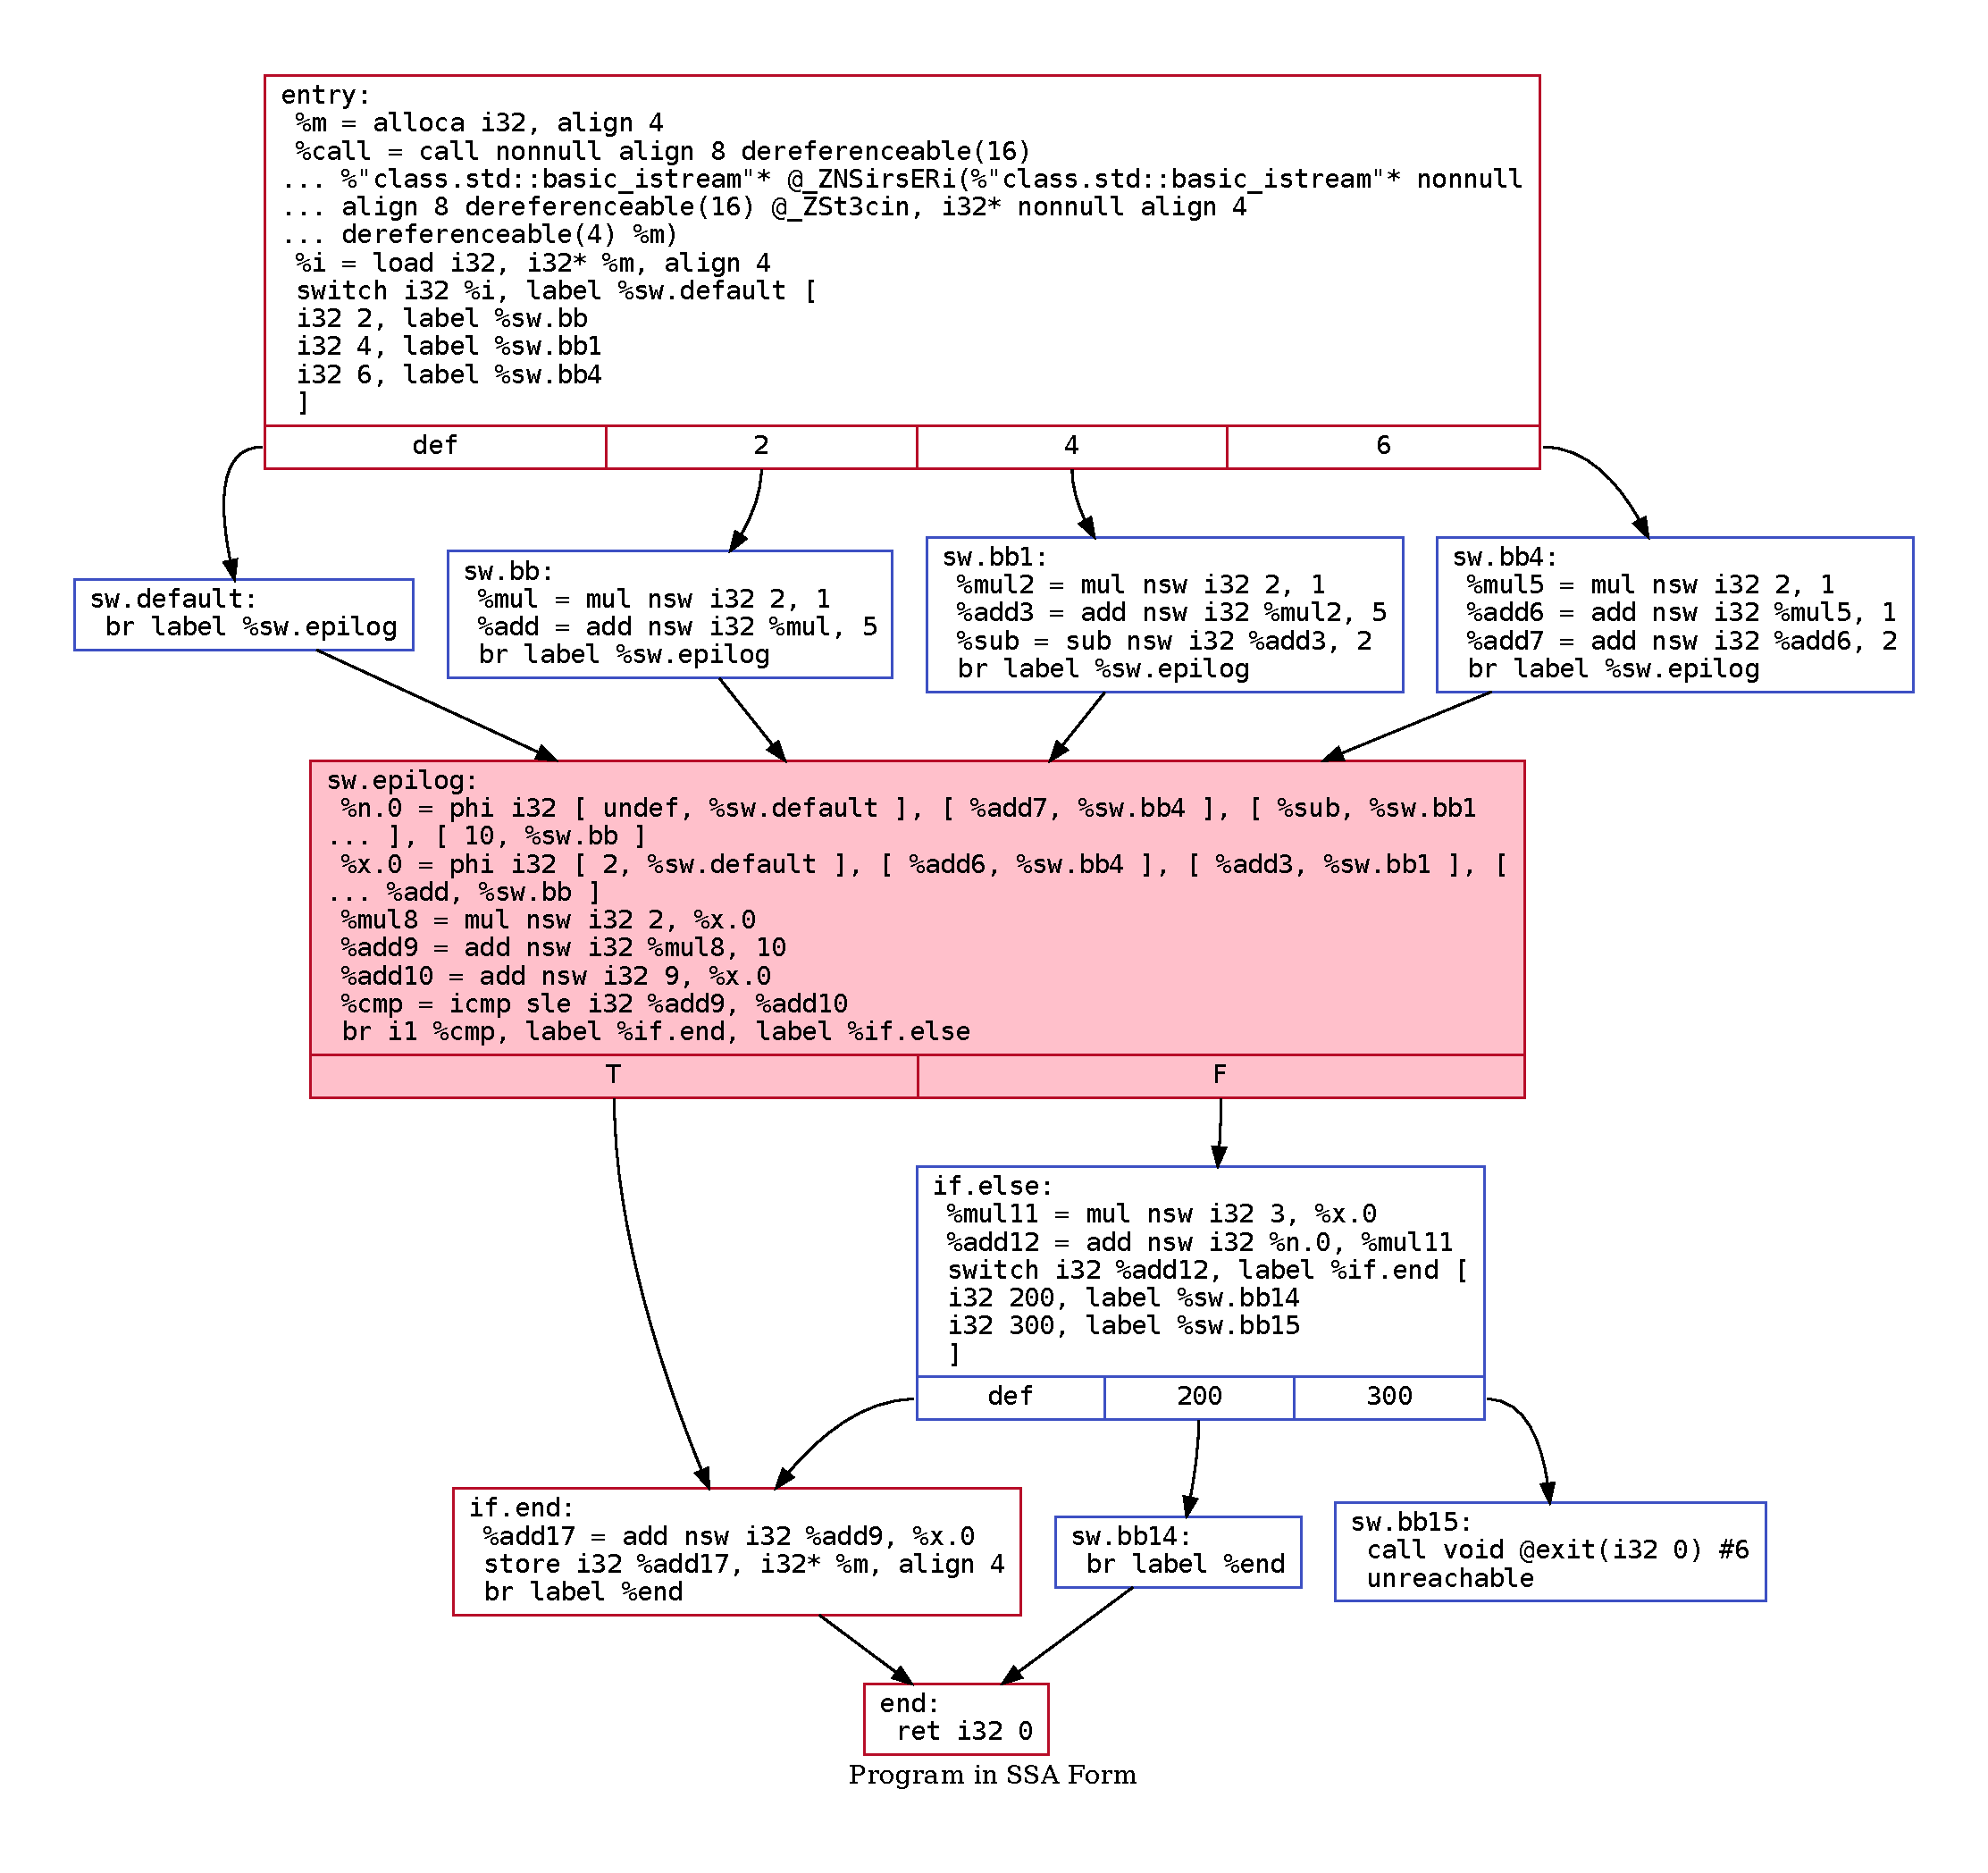
\includegraphics[width=9cm, height=8.35cm]{dotfiles/baseline.dot.pdf}
\end{frame}

\begin{frame}{Program in Hot Path SSA Form}
	\centering
	% HOT PATH SSA PICTURE. HOT PATH SSA, HPSSA 
	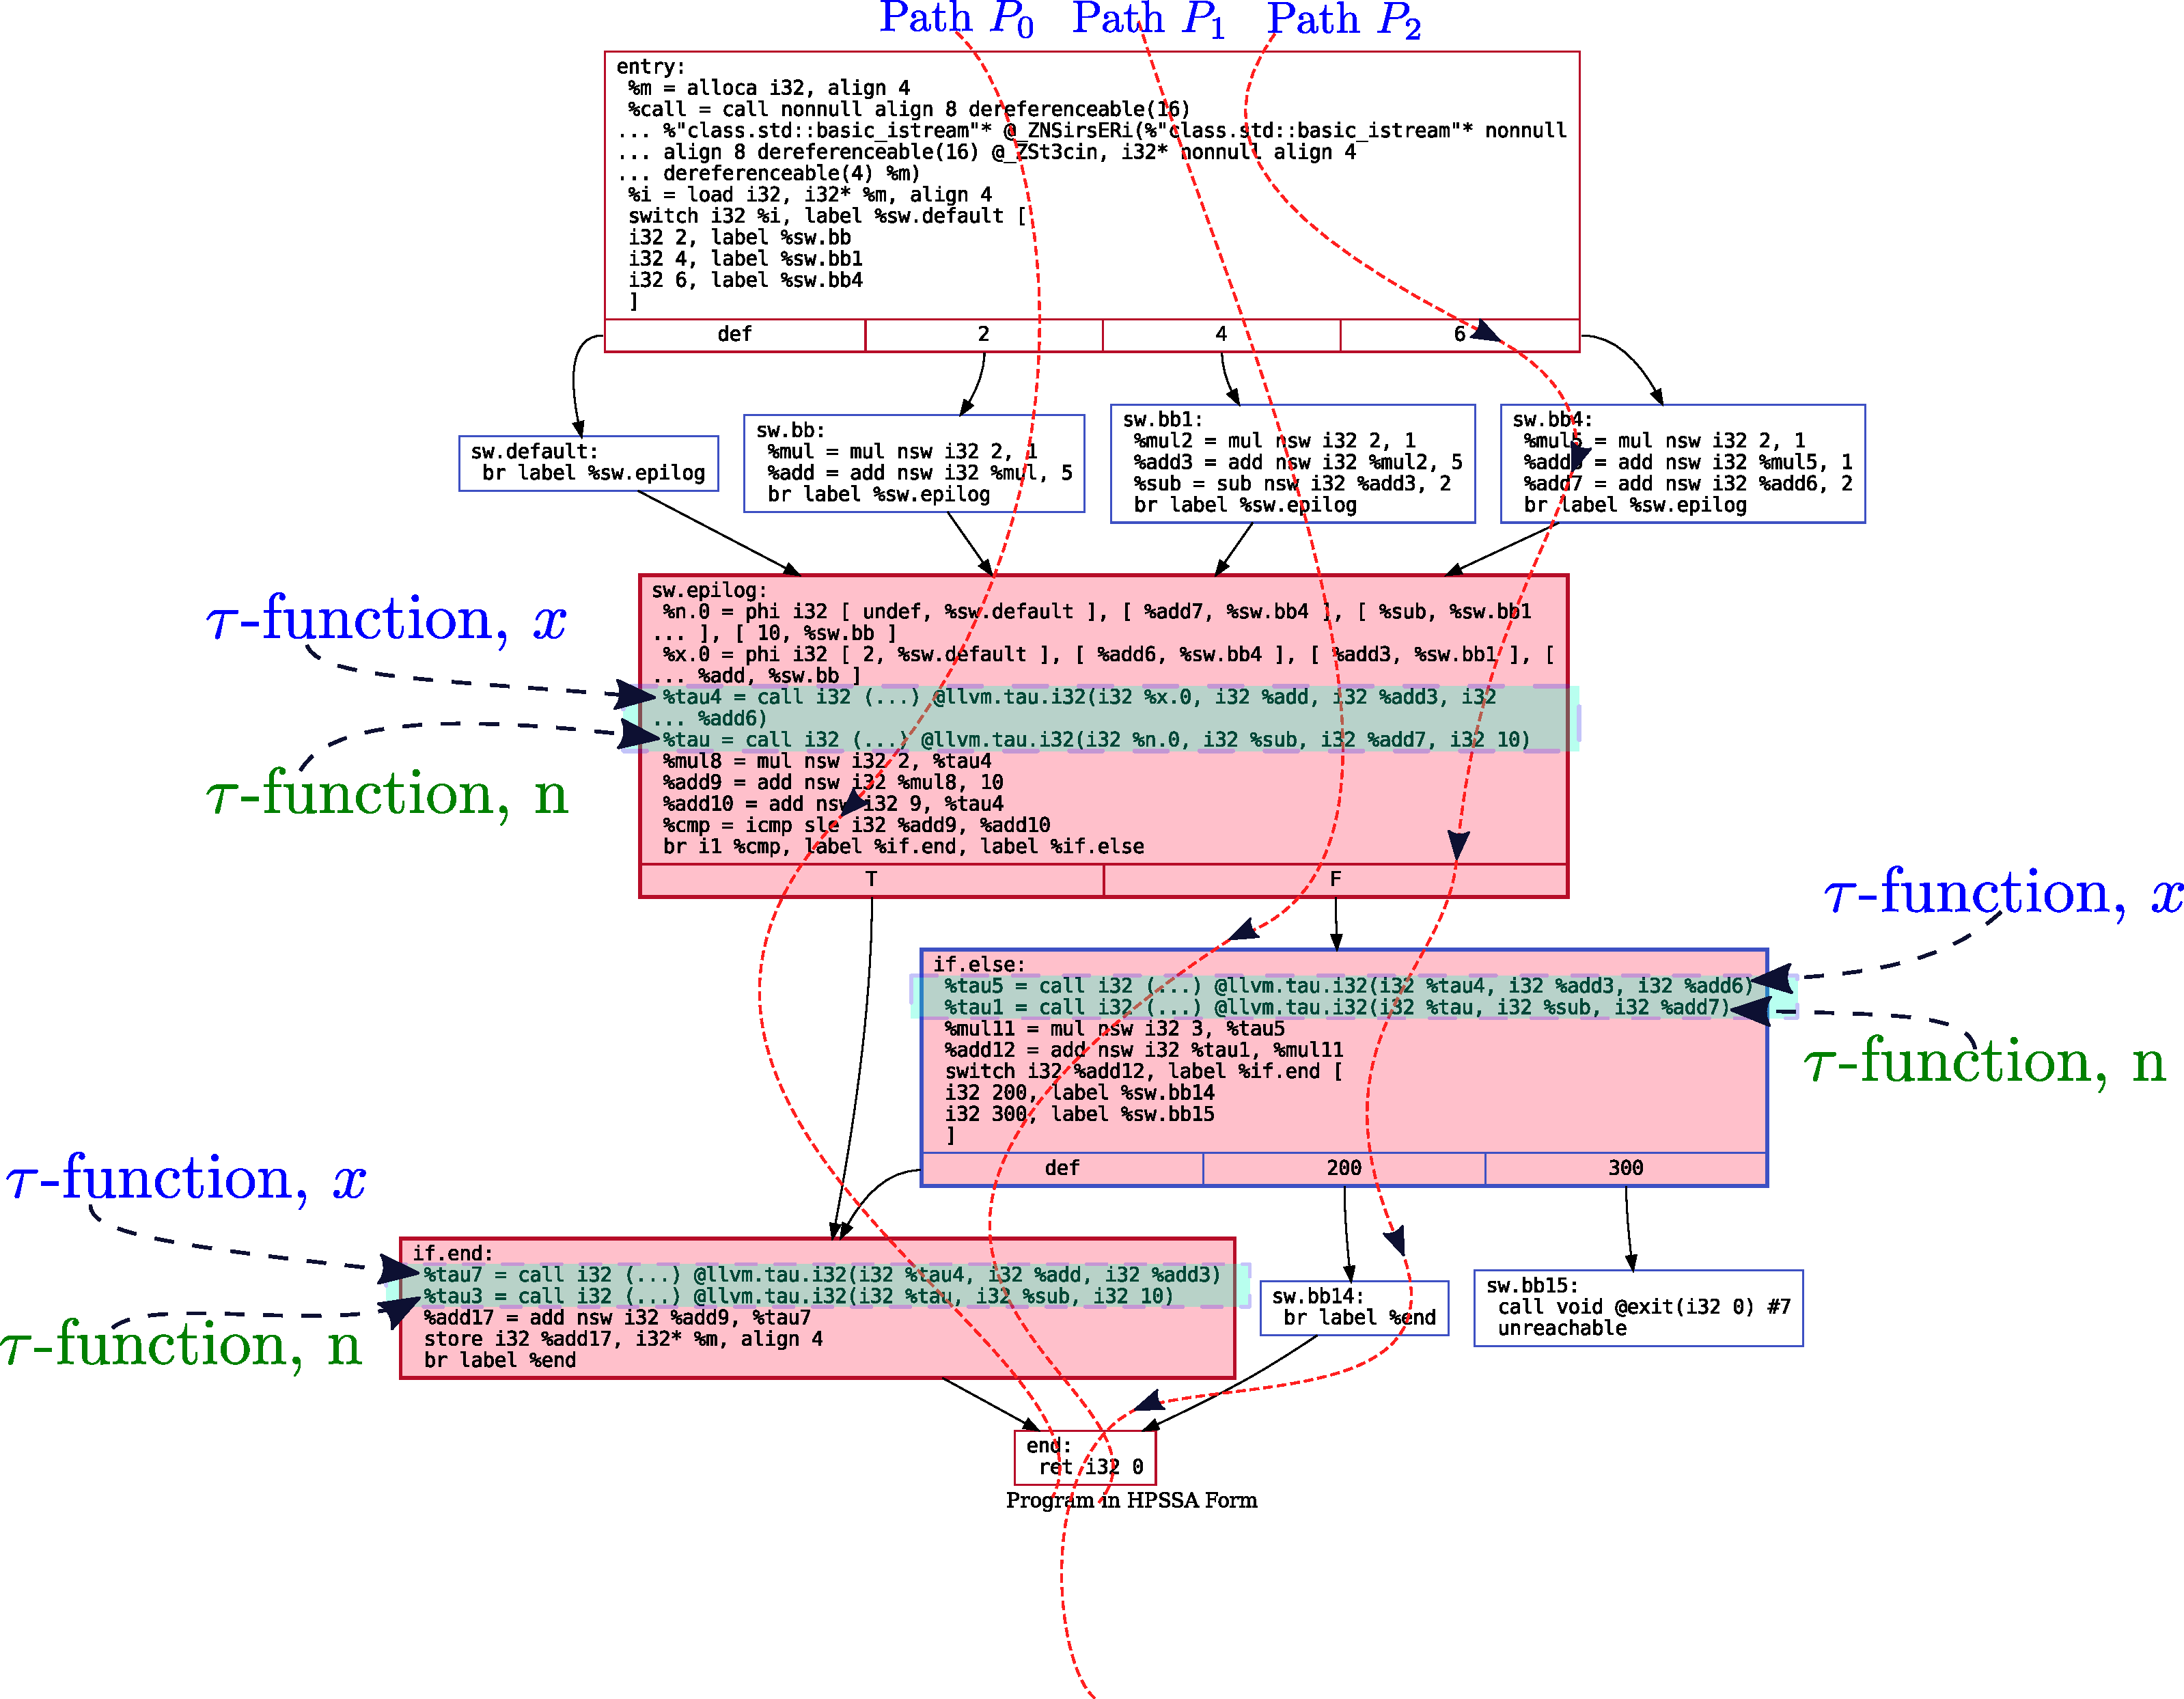
\includegraphics[width=12cm, height=8.95cm]{dotfiles/afterHPSSA.dot.pdf}
\end{frame}
\footnotesize

\end{document}